
\section{Experimental Studies}
\label{sec-expt}

In this section, we conduct four sets of experiments to evaluate (1) the generalization ability of our model, (2) the performance of our question oriented visual processing module (\kw{QVS} and \kw{VTP}), (3) the accuracy of our inference module (\kw{VI}), and (4) the overall performance of our model. \looseness =-1

\stitle{Experimental Setting}. %We report settings of experimental studies. 

\etitle{DataSet}. We used two data sets: (1) \kw{Soccer}~\cite{peixi2019} that we annotated; and (2) Visual-Genome~\cite{visualgenome}, one typical \vqa dataset. Over Visual-Genome dataset, we extracted 2852 images with subjects of baseball, tennis and soccer. 
For each dataset, we split it into two parts: Part$_I$, which accounts for 1/3 and used for testing, and Part$_{II}$ that accounts for 2/3 and used for training.   

\etitle{Questions}. We used two sets of questions: (1) the set of questions, listed in Table~\ref{table:questions} for \kw{Soccer}; and (2) another set of questions for Visual-Genome. The questions for Visual-Genome are generated as following. We went over questions posed on Visual-Genome, extracted three kinds of typical questions, \ie ``what'', ``how many'' and ``where'' as base questions, and constructed in total 1179 questions with base questions, where 869 for ``what'' type, 259 for ``how many'' type, and 51 for ``where'' type. 

%==========Table===================
\begin{table}[thb]
	\renewcommand{\arraystretch}{1}
	\begin{center}
		\footnotesize		
		\begin{tabular}{c|c|c}
			\Xhline{1pt}
			Id & Question                                           & Difficulty \\ \Xhline{0.7pt}
			%$Q_{nl_1}$  & Who is this image about?                         & Hard       \\ \hline
			$Q_{nl_1}$  & Who is holding the soccer?                         & Easy       \\ \hline
			$Q_{nl_2}$  & What is the uniform color of the referee?           & Easy       \\ \hline
			$Q_{nl_3}$  & Is there any referee in the image?                 & Easy       \\ \hline
			$Q_{nl_4}$  & Which team does the goalkeeper belong to?          & Medium       \\ \hline
			$Q_{nl_5}$  & Who is the defending team?                         & Medium       \\ \hline
			$Q_{nl_6}$  & Which part of the field are the players being now? & Hard       \\ \hline
			$Q_{nl_7}$  & How many players are there in the image?           & Hard     \\ \hline
			$Q_{nl_8}$  & Is this image about corner kick?                   & 
			\\ \hline
			$Q_{nl_9}$  & Is this image about free kick?                     & 
			\\ \hline
			$Q_{nl_{10}}$  & Is this image about kick off?                  & 
			\\ \hline
			$Q_{nl_{11}}$  &  Is this image about penalty kick?             &
			\\ \hline
			\eat{
			\multirow{2}{*}{$Q_{nl_8}$ }
			& Is this image about corner kick?           &  \multirow{2}{*}{\color{red}??}  \\ 
			& {\color{red}(If not, just list the correct one.)}  & \\ \hline
			
			\multirow{2}{*}{$Q_{nl_{9}}$}  &  Is this image about free kick?  &  \multirow{2}{*}{\color{red}??}    \\ 
			& {\color{red}(If not, just list the correct one.)}  &  \\ \hline
			
			\multirow{2}{*}{$Q_{nl_{10}}$}  &  Is this image about kick off?  &  \multirow{2}{*}{\color{red}??}    \\ 
			& {\color{red}(If not, just list the correct one.)}  &  \\ \hline
			
			\multirow{2}{*}{$Q_{nl_{11}}$}  &   Is this image about penalty kick?  &  \multirow{2}{*}{\color{red}??}    \\ 
			& {\color{red}(If not, just list the correct one.)}  &  \\ %\hline
			\Xhline{1pt}
			}
		\end{tabular}
		\caption{A set of questions}
		\label{table:questions}
	\end{center}
\end{table}
%==========Table===================


\subsection{Generalization Ability of the Model}

To show the generalization ability of our model, we compared accuracy of our model with state-of-the-art methods CNN+LSTM~\cite{VQA}, HieCoAttenVQA~\cite{Lu2016Hie} and Learning2Reason~\cite{hu2017learning}, via changes of training data. For comparison purpose, we enrich training data with those questions taking the same semantic meaning. For example, besides $Q_{nl5}$, we add following questions: \textit{Who is attacking team?}, \textit{"What is the uniform color of the defending team?"} and \textit{"What is the uniform color of the attacking team?"}, that have the same semantic meaning as $Q_{nl5}$ in training data. As shown in Table~\ref{table:genralization}, our model always outperforms others, and moreover, is influenced least by varied training data, than other methods. The reason is that all the visual task selection is question oriented, which leads to unfixed network structure, also, the graph-based method preserves better reasoning capability, comparing with memorizing statistic correlations between images and answers.


\eat{
To test the generalization of our method, we enlarge the training set by more various question with same meaning. For instance, the original question of $Q_{nl5}$ is \textit{"Who is the defending team?"}, we add three more similar question asking \textit{Who is attacking team?}, \textit{"What is the uniform color of the defending team?"} and \textit{"What is the uniform color of the attacking team?"}. Unlike state-of-the-art methods answering questions in~\cite{peixi2019}, adding generalization and variation in question would not dramatically change the performance, it is because the structure is not fixed, all the visual task selection is query oriented. For~\cite{hu2017learning}, even though the network is not fixed, the answering part is based on neural network, and essentially it also learns the statically correlation, which leads to the weakness in logical reasoning. The result is is shown in Table~\ref{table:genralization}.
}

\begin{table}[h]
	\small
	\begin{tabular}{|l|l||l|l|}
		\hline
		\multicolumn{2}{|l||}{Various Training Questions} & \multicolumn{2}{l|}{Original Training Questions} \\ \hline \hline
		Methods                  & Acc(\%)            & Methods                   & Acc(\%)             \\ \hline
		CNN+LSTM                    & 28.14              & CNN+LSTM                     & 46.40               \\ \hline
		HieCoAttenVQA               & 31.92              & HieCoAttenVQA                & 49.11               \\ \hline
		Learning2Reason             & 38.00              & Learning2Reason              & 51.08               \\ \hline
		Ours                        & 64.02              & Ours                         & 66.75               \\ \hline
	\end{tabular}
	\caption{Generalization ability of our model} \label{table:genralization}
\end{table}


\subsection{Performance of Visual Processing}

Efficiency is one crucial factor to evaluate the performance of a \vqa model. 
In light of this, we evaluate the running time over accuracy by using state-of-the-art methods CNN+LSTM~\cite{VQA} HieCoAttenVQA~\cite{Lu2016Hie}, Learning2Reason~\cite{hu2017learning} and AllTasks~\cite{peixi2019}. To measure the efficiency of \vqa models, we use ``CPU Time'' to represent the total running time of entire progress of question answering. 

The results shown in \Cref{fig:TimevsAcc} tell us that: (1) state-of-the-art methods perform efficiently, with running time less than 300 milliseconds, while their accuracy are all below 40\%, showing that the methods are not applicable in practice; (2) AllTasks always has the highest and steady accuracy, \eg 65.86\%, since it processes all the visual related tasks without selection, paying the price of unexpected and long running time; and (3) our module finds a balance between efficiency and accuracy. For example, with $\gamma=0.99$, our reinforcement learning based module spends, on average, 680 ms to answer questions, with accuracy 64.02\%, which is 35.88\%, 32.10\% and 26.02\% higher than that of CNN+LSTM, HieCoAttenVQA, and Learning2Reason, respectively. Moreover, when running time decreases, the accuracy decreases either, which is as expected.

\begin{figure}[h]
	\begin{center}
		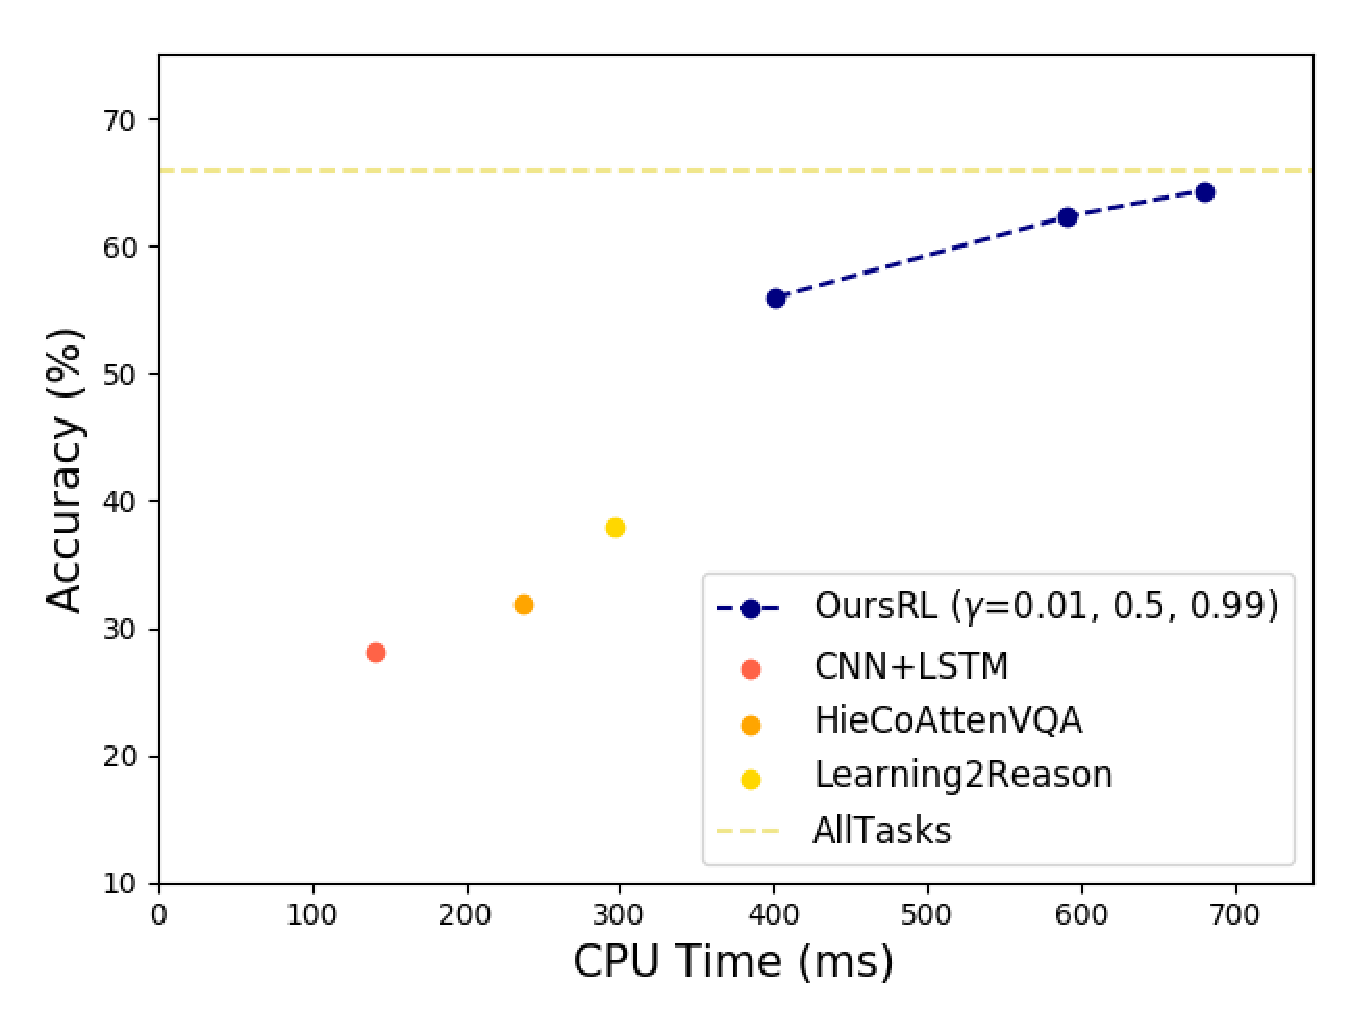
\includegraphics[width=0.75\linewidth]{figures/TimevsAcc.eps}
	\end{center}
	\vspace{-3ex}
	\caption{Balance between running time and accuracy}
	\vspace{-2ex}
	\label{fig:TimevsAcc}
\end{figure}


\eat{
	\Cref{tab:AccuracyCmp} lists the time cost and accuracy results among different approaches. For CNN+LSTM, HieCoAttenVQA, and Learning2Reason, their systems work quite efficient with responding time less than 300ms. But the accuracies of these three approaches are lower than 40\%, which is unacceptable. Whereas, the system similar to \cite{peixi2019} outperforms all other methods and reaches 65.86\% accuracy, but it costs much more time. Our approach is able to keep balance between effectiveness and efficiency. For effectiveness, our approach achieves 64.02\% accuracy, which is 35.88\%, 32.10\% and 26.02\% higher than results of CNN+LSTM, HieCoAttenVQA, and Learning2Reason, respectively. For efficiency, our approach can reduce the inference time by choosing a small value of $\gamma$.
	
	
	We compare our approach to the state-of-the-art systems, \ie CNN+LSTM~\cite{VQA} HieCoAttenVQA~\cite{Lu2016Hie}, and Learning2Reason~\cite{hu2017learning}. 
	
	%==========Table===================
	\begin{table}[htbp]
		\renewcommand{\arraystretch}{1}
		\begin{center}
			\small		
			\begin{tabular}{c|*{2}{c}}
				\Xhline{1pt}
				& Time (ms)  & Accuracy (\%) \\ \Xhline{0.7pt}
				CNN+LSTM  &  141  &  28.14\\
				HieCoAttenVQA  &  237  &  31.92\\
				Learning2Reason  &  297  &  38.00\\
				Ours (Without RL)  &  N/A  &  65.85\\
				Ours ($\gamma=0.01$)  &  401  &  55.92\\
				Ours ($\gamma=0.50$)  &  591  &  62.29\\
				Ours ($\gamma=0.99$)  &  680  &  64.02\\
				\Xhline{1pt}
			\end{tabular}
			\caption{Inference time and accuracy comparison.}
			\label{tab:AccuracyCmp}
		\end{center}
	\end{table}
	%==========Table===================
}


\subsection{Performance of Inference} 
\eat{
	\begin{figure}[tb!]
		\centering
		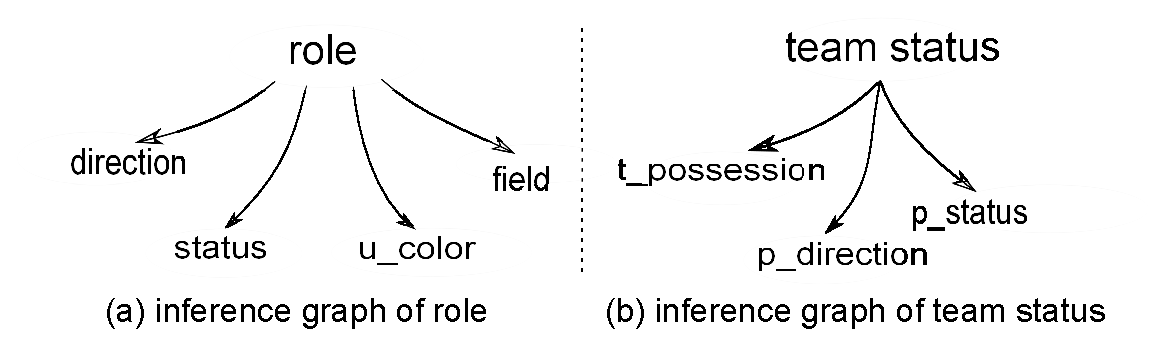
\includegraphics[width=\columnwidth]{PredictNB.eps}
		\vspace{-2ex}
		\caption{Inference graphs}
		\vspace{-2ex}
		\label{fig:inferGraph}
	\end{figure}
}

Accuracy is another crucial performance criteria of \vqa systems. In contrast to end-to-end systems, the accuracy of our model is partly influenced by the inference quality. Hence, it is of great importance to see how accuracy is influenced by our inference module (\kw{VI}). Prior work~\cite{peixi2019} already showed performance of their inference module \wrt a set of fixed questions on Soccer dataset. Here, we learn an inference graph for questions $Q_{nl8},Q_{nl9},Q_{nl10}$ and $Q_{nl11}$ regarding field scene from Soccer dataset, and a set of inference graphs for answering questions on Visual-Genome dataset. \looseness=-1

To evaluate accuracy, we follow F-measure~\cite{Fmeasure}, and define our accuracy metric as following:


\noindent $\kw{Acc}=2\cdot (\kw{recall}\cdot \kw{precision})~/~(\kw{recall}+\kw{precision})$;

\noindent $\kw{recall}=\#\kw{true}\_\kw{value}\_\kw{inferred}~/~\#\kw{true}\_\kw{value}\_\kw{instance}$;

\noindent $\kw{precision}=\#\kw{true}\_\kw{value}\_\kw{inferred}~/~\#\kw{inferred}\_\kw{instance}$.


Here $\#\kw{true}\_\kw{value}\_\kw{inferred}$ is the number of all the instances, whose attribute $A$ is inferred correctly as $``v"$,  $\#\kw{true}\_\kw{value}\_\kw{instance}$ is the number of all the instances with attribute $A$ of value $``v"$, and $\#\kw{inferred}\_\kw{instance}$ indicates the total number of instances whose attribute $A$ is inferred as $``v"$. \looseness=-1




\eat{
\stitle{Accuracy of Role}. 

Based on questions and image characteristics, four variables including $direction$, $status$, $field$, and $unique\_color$ (abbr. $u\_color$) are adopted to calculate conditional probabilities. The inference graph is shown in \Cref{fig:inferGraph}. Note that the domain of variables $direction$, $status$ and $field$ are given in {\color{red}Table ????}, while variable $u\_color$ can have one of two values, to indicate whether a person object has the unique uniform color (=``$U$'') or not (=``$M$'').

%==========Table===================
\begin{table}[htbp]
	\renewcommand{\arraystretch}{1}
	\begin{center}
		\small		
		\begin{tabular}{c|*{3}{r}}
			\Xhline{1pt}
			Role & Precision  & Recall  & Acc \\ \Xhline{0.7pt}
			Goalkeeper  &  94.4  &  85.5  &  89.8\\
			Referee  &  87.4  &  82.8  &  85.0\\
			Player  &  98.8  &  99.3  &  99.0\\
			\Xhline{1pt}
		\end{tabular}
	\caption{Inference accuracy of role (\%).}
	\label{tab:InferAccRole}
	\end{center}
\end{table}
%==========Table===================

Using the conditional probabilities, $VI$ {\color{red}(???)} infers role of each person object. The inference accuracy is shown in \Cref{tab:InferAccRole}. It is easy to find that the inference accuracy for role player reaches 99\%, which is highest among all roles. And the accuracy for different roles are all above 85\%.

\stitle{Accuracy of Team Status}

%===================== figure ============
\begin{figure}[!bth]
	%\scriptsize
	\centering	
	\begin{minipage}[b]{\linewidth}
		\centerline{\includegraphics[width=0.5\linewidth]{example-image-a}}
	\end{minipage}\hfill
	\caption{Attributes of team inference graph.}
	\label{fig:AtribTeamGraph}
\end{figure}
%===================== figure ============

%==========Table===================
\begin{table}[htbp]
	\renewcommand{\arraystretch}{1}
	\begin{center}
		\small		
		\begin{tabular}{c|*{3}{r}}
			\Xhline{1pt}
			 Team Status & Precision  & Recall  & Acc \\ \Xhline{0.7pt}
			Defending  & 89.8 &	74.2 &	81.3\\
			Attacking  &  79.1 & 	92.1 &	85.1\\
			\Xhline{1pt}
		\end{tabular}
		\caption{Inference accuracy of team status (\%).}
		\label{tab:InferAccTeam}
	\end{center}
\end{table}
%==========Table===================

\Cref{tab:InferAccTeam} gives the performance of our approach for inferring team status. The accuracy of defending and attacking are above 80\%. To be specific, the accuracy for inferring if a team is attacking achieves 85.1\%, which is higher than the inference accuracy for defending status detection by 3.8\%.
}


%===================== figure ============
\begin{figure}[!bth]
	%\scriptsize
	\centering	
	\begin{minipage}[b]{\linewidth}
		\centerline{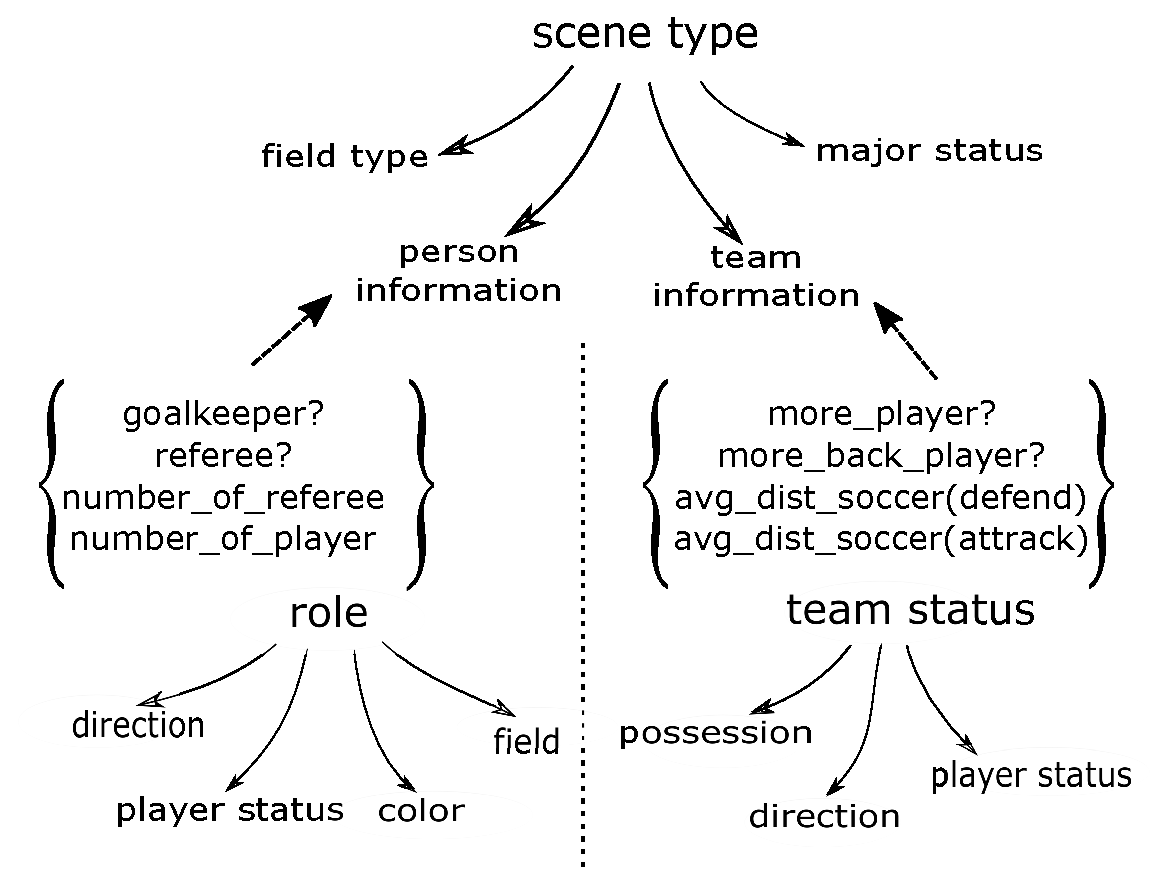
\includegraphics[width=1\linewidth]{attribtes_infGraph}}
	\end{minipage}\hfill
	\caption{Attributes of scene inference graph.}
	\label{fig:AtribSceneGraph}
\end{figure}
%===================== figure ============


\stitle{Accuracy of Field Scene}. We choose four typical field scenes, \ie corner kick, free kick, penalty kick and kick-off, as  which have distinct scene features. Practically, (1) corner kick scene always shows that a single player kicks the ball within a one-yard radius of the corner flag and most of players gather at the penalty field. (2) Free kick happens with a defensive wall mostly. (3) It is much typical for the penalty kick scene because most of players are out of penalty area except the penalty kicker and goalkeeper with football in the penalty spot. (4) For kick-off scene, the soccer appears in the center spot and is surrounded by players from two opposing teams. Based on these observations, we design an inference graph which is shown in \Cref{fig:AtribSceneGraph}.

Using inference graph shown in Fig.~\ref{fig:AtribSceneGraph}, we have results
showing accuracy of inference. 
%Inference results are indicated in \Cref{tab:InferAccField} based on inference graph in \Cref{fig:AtribSceneGraph}. 
As can be seen, the inference accuracy of corner kick, free kick, kick-off and penalty kick are 59.57\%, 63.16\%, 85.94\% and 60.00\%, respectively, among which the scene of kick off gains the highest inference accuracy.
 

%==========Table===================
\begin{table}[htbp]
	\renewcommand{\arraystretch}{1}
	\begin{center}
		\small		
		\begin{tabular}{c|*{3}{r}}
			\Xhline{1pt}
			Scene Type & Precision  & Recall  & Acc \\ \Xhline{0.7pt}
			Corner-kick &  59.57  &  68.29  &  63.64\\
			Free-kick  &  63.16  &  58.54  &  60.76\\
			Kick-off &  85.94  &  82.09  &  83.97\\
			Penalty-kick  &  60.00  &  60.00  &  60.00\\
			\Xhline{0.7pt}
			Avg.  &  71.28  &  70.73  &  70.89\\
			\Xhline{1pt}
		\end{tabular}
	\caption{Inference accuracy of four typical scenes (\%).
		% Here ``Co'', ``Fr'', ``Ki'' and ``Pe'' indicate corner kick, free kick, penalty kick and kick-off, respectively.
	}
	\label{tab:InferAccField}
	\end{center}
	\vspace{-3ex}
\end{table}
%==========Table===================


In addition, we compare our approach with NuSVC, MLP, and AdaBoost in \Cref{tab:AccFieldCmp}. The results show that the average accuracy of our approach is higher than that of NuSVC and AdaBoost by 4.49\% and 5.97\% respectively, and slightly better than that of MLP.

%==========Table===================
\begin{table}[htbp]
	\renewcommand{\arraystretch}{1}
	\begin{center}
		\small		
		\begin{tabular}{c|*{3}{r}}
			\Xhline{1pt}
			 & Precision  & Recall  & Acc \\ \Xhline{0.7pt}
			NuSVC  &  68.30  &  65.85  &  66.40\\
			MLP  &  70.80  &  \textbf{70.73}  &  70.32\\
			AdaBoost  &  65.50  &  65.24  &  64.92\\ %\Xhline{0.7pt}
			Ours  &  \textbf{71.28}  &  \textbf{70.73}  &  \textbf{70.89}\\
			\Xhline{1pt}
		\end{tabular}
	\caption{Accuracy comparison of field scene (\%)}
	\label{tab:AccFieldCmp}
	\end{center}
	\vspace{-3ex}
\end{table}
%==========Table===================



%\stitle{Accuracy of Kick-Off}. {\color{red} SHOW INFERENCE GRAPH AND RESULT TABLE!}
%
%\stitle{Accuracy of Penalty Kick}. {\color{red} SHOW INFERENCE GRAPH AND RESULT TABLE!}
%
%\stitle{Accuracy of Corner Kick}. {\color{red} SHOW INFERENCE GRAPH AND RESULT TABLE!}
%
%\stitle{Accuracy of Attacking Free Kick}. {\color{red} SHOW INFERENCE GRAPH AND RESULT TABLE!}
%
%\stitle{Accuracy of Balls}. {\color{red} Over new dataset. SHOW INFERENCE GRAPH AND RESULT TABLE!}

\subsection{Overall Performance}
\label{sec-overall-performance}
%We use the same question setting as~\cite{peixi2019}, compared the following state-of-the-art methods: \cite{VQA},and~\cite{hu2017learning} with our method ($\gamma$=0.99), the overall performance is shown in Table~\ref{table:stateofart}. 

We compare our approach with the following state-of-the-art methods: CNN+LSTM, HieCoAttenVQA, and Learn2Reason, using Soccer and Visual-Genome dataset. 
Table~\ref{table:stateofartSoc} lists results on Soccer. We find that (1) the average accuracy of our approach is higher than that of CNN+LSTM, HieCoAttenVQA and Learn2Reason by 20.35\%, 17.64\% and 15.67\%,  respectively; (2) our approach is typically effective in answering hard problems, \eg with improvement over 60\% for $Q_{nl6}$. 
Consider that questions $Q_{nl8}-Q_{nl11}$ are all about field scene, while more than 90\% images of Soccer dataset are categorized as normal scene. For the fair comparison, we extract images that are categorized as one of four field scenes, and apply our approach over this subset of dataset. As shown in Table~\ref{table:stateofartSoc}, our approach substantially outperforms others, which further verifies the advantage our approach preserves. 
Results on Visual-Genome are given in Table~\ref{table:stateofartVisGen}, from which we find: (1) for ``what'' and ``where'' questions, Learn2Reason performs best, while performances of four methods are quite close; (2) for ``how many'' questions, our method performs much better than others; and (3) the average accuracy our method  surpasses CNN+LSTM, HieCoAttenVQA and Learn2Reason by 12.93\%, 11.74\% and 9.7\%, respectively, which further verifies its advantage. 
\eat{
To evaluate the generalization of the proposed scheme, we measure its accuracy on Visual Genome Dataset. Results in \Cref{table:stateofartVisGen} show that our approach can handle different types of questions, and the overall performance of our approach surpasses CNN+LSTM, HieCoAttenVQA and Learn2Reason by 12.93\%, 11.74\% and 9.7\%, respectively.
}
\eat{
The results are listed in \Cref{table:stateofartSoc}. The average accuracy using our approach is higher than that of CNN+LSTM, HieCoAttenVQA and Learn2Reason by 20.35\%, 17.64\% and 15.67\%,  respectively. 
}

%==========Table===================
\begin{table}[htbp]
	\renewcommand{\arraystretch}{1}
	\begin{center}
		\small		
		\begin{tabular}{c|*{4}{c}}
			\Xhline{1pt}
			& CNN+LSTM & HieCoAtten & Learn2Reason & Ours \\ \Xhline{0.7pt}
			$Q_{nl1}$ & 44.23    & 43.62         & 31.12        & \textbf{64.86} \\ 
			$Q_{nl2}$ & 71.31    & \textbf{77.66}         & 9.4          & 63.74 \\ 
			$Q_{nl3}$ & 74.58    & \textbf{83.78}         & 83.21        & 70.00 \\ 
			$Q_{nl4}$ & 40.48    & 39.29         & 51.92        & \textbf{62.14} \\ 
			$Q_{nl5}$ & 49.19    & 49.90         & 30.78        & \textbf{62.58} \\ 
			$Q_{nl6}$ & 20.56    & 18.70         & 30.0         & \textbf{93.33} \\ 
			$Q_{nl7}$ & 11.08    & 12.63         & 36.69        & \textbf{50.60} \\\Xhline{0.7pt} 
			$Q_{nl8}$ &     &           &          &   \\
			$Q_{nl9}$ &     &           &          &   \\
			$Q_{nl10}$ &      &           &          &   \\
			$Q_{nl11}$ &      &           &          &   \\ \Xhline{0.7pt} 
			Avg.       & 46.40    & 49.11         & 51.08        & \textbf{66.75} \\
			\Xhline{1pt}
		\end{tabular}
	\caption{Performance comparison on Soccer dataset (\%).}
	\label{table:stateofartSoc}
	\end{center}
	\vspace{-3ex}
\end{table}
%==========Table===================


%==========Table===================
\begin{table}[htbp]
	\renewcommand{\arraystretch}{1}
	\begin{center}
		\small		
		\begin{tabular}{c|*{4}{c}}
			\Xhline{1pt}
			& CNN+LSTM & HieCoAtten & Learn2Reason & Ours \\ \Xhline{0.7pt}
			$Q_{t1}$  &  63.72  &  64.83  &  \textbf{67.12}  &  65.59\\
			$Q_{t2}$  &  22.87  &  24.52  &  25.04  &  \textbf{82.87}\\
			$Q_{t3}$  &  36.96  &  37.89  &  \textbf{40.12}  &  34.16\\ \Xhline{0.7pt} 
			Avg.       &  50.48  &  51.67  &  53.71  &  \textbf{63.41}\\
			\Xhline{1pt}
		\end{tabular}
		\caption{Performance comparison on Visual Genome dataset (\%).}
		\label{table:stateofartVisGen}
	\end{center}
	\vspace{-3ex}
\end{table}
%==========Table===================

